%%%%%%%%%%%%%%%%%%%%%%%%%%%%%%%%%%%%%%%%%%%%%%%%%%%%%%%%%%%%%%%%%%%%%%%%%%%%%%%%%%%%%%%%%%%%%%%%%%%%%%%
%%%%%%%%%%%%%% Template de Artigo Adaptado para Trabalho de Diplomação do ICEI %%%%%%%%%%%%%%%%%%%%%%%%
%% codificação UTF-8 - Abntex - Latex -  							     %%
%% Autor:    Fábio Leandro Rodrigues Cordeiro  (fabioleandro@pucminas.br)                            %% 
%% Co-autor: Prof. João Paulo Domingos Silva, Harison da Silva e Anderson Carvalho                   %%
%% Revisores normas NBR (Padrão PUC Minas): Helenice Rego Cunha e Prof. Theldo Cruz                  %%
%% Versão: 1.1     18 de dezembro 2015                     	                                     %%
%%%%%%%%%%%%%%%%%%%%%%%%%%%%%%%%%%%%%%%%%%%%%%%%%%%%%%%%%%%%%%%%%%%%%%%%%%%%%%%%%%%%%%%%%%%%%%%%%%%%%%%


\documentclass[a4paper,12pt,Times]{article}
\usepackage{abakos}  %pacote com padrão da Abakos baseado no padrão da PUC
\usepackage{ragged2e}
\usepackage{float}
\usepackage{pdfpages}
%%%%%%%%%%%%%%%%%%%%%%%%%%%
%Capa da revista
%%%%%%%%%%%%%%%%%%%%%%%%%%

%\setcounter{page}{80} %iniciar contador de pagina de valor especificado

\newcommand{\monog}{ 
\begin{center}
Compilador para a linguagem de programação L    
\end{center}}
\newcommand{\tipo}{Artigo }  % Especificar a seção tipo do trabalho: Artigo, Resumo, Tese, Dociê etc
\newcommand{\origem}{Brasil }
\newcommand{\editorial}{Belo Horizonte, p. 01-05, mai. 2019}  % p. xx-xx – páginas inicial-final do artigo
\newcommand{\lcc}{\scriptsize{Licença Creative Commons Attribution-NonCommercial-NoDerivs 3.0 Unported}}

%%%%%%%%%%%%%%%%%INFORMAÇÕES SOBRE AUTOR PRINCIPAL %%%%%%%%%%%%%%%%%%%%%%%%%%%%%%%

\newcommand{\AutorA}{Vinicius Francisco da Silva}
\newcommand{\funcaoA}{}
\newcommand{\emailA}{vinicius.silva.1046664@sga.pucminas.br}
\newcommand{\cursA}{Aluno do Programa de Graduação em Ciência da Computação}
% 
% Definir macros para o nome da Instituição, da Faculdade, etc.
\newcommand{\univ}{Pontifícia Universidade Católica de Minas Gerais}

\newcommand{\keyword}[1]{\textsf{#1}}

\begin{document}
% %%%%%%%%%%%%%%%%%%%%%%%%%%%%%%%%%%
% %% Pagina de titulo
% %%%%%%%%%%%%%%%%%%%%%%%%%%%%%%%%%%

\begin{center}

\includegraphics[scale=0.2]{figuras/brasao.jpg} \\
PONTIFÍCIA UNIVERSIDADE CATÓLICA DE MINAS GERAIS \\
Instituto de Ciências Exatas e de Informática \\
Departamento de Ciência da Computação \\
Disciplina: Compiladores

% \vspace{1.0cm}

\end{center}

 \vspace{0cm} {
 	\singlespacing \Large{\monog \symbolfootnote[1]{Trabalho apresentado para a disciplina de compiladores.} \\ }
 }

\vspace{1.0cm}

\begin{flushright}
\singlespacing 
\normalsize{\AutorA \footnote{\funcaoA \cursA, \origem -- \emailA . }}
%deixar com o valor `0` e usar o '*' no inicio da frase
% \symbolfootnote[0]{Artigo recebido em 10 de julho de 1983 e aprovado em 29 de maio 2012}
\end{flushright}
\thispagestyle{empty}

\vspace{1.0cm}

%\begin{abstract}
%\noindent

%\\\textbf{\keyword{Palavras-chave: }} 
%\end{abstract}

%%%%%%%%%%%%%%%%%%%%%%%%%%%%%%%%%%%%%%%%%%%%%%%%%%%%%%%%%

\selectlanguage{brazilian}
 \onehalfspace  % espaçamento 1.5 entre linhas
 \setlength{\parindent}{1.25cm}

%%%%%%%%%%%%%%%%%%%%%%%%%%%%%%%%%%%%%%%%%%%%%%%%%
%% INICIO DO TEXTO
%%%%%%%%%%%%%%%%%%%%%%%%%%%%%%%%%%%%%%%%%%%%%%%%%

%%%%%%%%%%%%%%%%%%%%%%%%%%%%%%%%%%%%%%%%%%%%%%%%%%%%%%%%%%%%%%%%%%%%%%%%%%%%%%%%%%%%%%%%%%%%%%%%%%%%%%%
%%%%%%%%%%%%%% Template de Artigo Adaptado para Trabalho de Diplomação do ICEI %%%%%%%%%%%%%%%%%%%%%%%%
%% codificação UTF-8 - Abntex - Latex -  							     %%
%% Autor:    Fábio Leandro Rodrigues Cordeiro  (fabioleandro@pucminas.br)                            %% 
%% Co-autores: Prof. João Paulo Domingos Silva, Harison da Silva e Anderson Carvalho		     %%
%% Revisores normas NBR (Padrão PUC Minas): Helenice Rego Cunha e Prof. Theldo Cruz                  %%
%% Versão: 1.1     18 de dezembro 2015                     %%
%%%%%%%%%%%%%%%%%%%%%%%%%%%%%%%%%%%%%%%%%%%%%%%%%%%%%%%%%%%%%%%%%%%%%%%%%%%%%%%%%%%%%%%%%%%%%%%%%%%%%%%
\section{Alfabeto $\Sigma$} 
\begin{table}[!h]
\centering
\caption{Elementos do alfabeto $\Sigma$}
\vspace{0.2cm}
\begin{tabular}{r}
 
Elemento \\ % Note a separação de col. e a quebra de linhas
\hline                               % para uma linha horizontal
\textit{\textbf{final}}\\
\textit{\textbf{else}}\\
\textit{\textbf{(}}\\
\textit{\textbf{<=}}\\
\textit{\textbf{;}}\\
\textit{\textbf{write}}\\
\textit{\textbf{int}}\\
\textit{\textbf{\&\&}}\\
\textit{\textbf{)}}\\
\textit{\textbf{,}}\\
\textit{\textbf{begin}}\\
\textit{\textbf{writeln}}\\
\textit{\textbf{byte}}\\
\textit{\textbf{||}}\\
\textit{\textbf{<}}\\
\textit{\textbf{+}}\\
\textit{\textbf{endwhile}}\\
\textit{\textbf{TRUE}}\\
\textit{\textbf{string}}\\
\textit{\textbf{!}}\\
\textit{\textbf{>}}\\
\textit{\textbf{-}}\\
\textit{\textbf{endif}}\\
\textit{\textbf{FALSE}}\\
\textit{\textbf{while}}\\
\textit{\textbf{<-}}\\
\textit{\textbf{!=}}\\
\textit{\textbf{*}}\\
\textit{\textbf{endelse}}\\
\textit{\textbf{boolean}}\\
\textit{\textbf{if}}\\
\textit{\textbf{=}}\\
\textit{\textbf{>=}}\\
\textit{\textbf{/}}\\
\textit{\textbf{readln}}\\
\end{tabular}
\end{table}


\section{\esp Lexemas e Padrão de formação}
\begin{table}[!h]
\centering
\caption{Lexema x Padrão de formação}
\vspace{0.2cm}
\begin{tabular}{r|lr}
 
Posi{\c c}{\~a}o & Lexema & Padr{\~a}o de Forma{\c c}{\~a}o \\ % Note a separação de col. e a quebra de linhas
\hline                               % para uma linha horizontal
1 & final & final\\
2 & else & else\\
3 & ( & ( \\
4 & <= & <= \\
5 & ; & ; \\
6 & write & write\\
7 & int & int\\
8 & \&\& & \&\& \\
9 & ) & ) \\
10 & , & , \\
11 & begin & begin\\
12 & writeln & writeln\\
13 & byte & byte\\
14 & || & || \\
15 & < & < \\
16 & + & + \\
17 & endwhile & endwhile\\
18 & TRUE & TRUE \\
19 & string & string\\
20 & ! & ! \\
21 & > & > \\
22 & - & - \\
23 & endif & endif\\
24 & FALSE & FALSE \\
25 & while & while\\
26 & <- & <- \\
27 & != & !=  \\
28 & * & * \\
29 & endelse & endelse\\
30 & boolean & boolean\\
31 & if & if\\
32 & = & = \\
33 & >= & >= \\
34 & / & / \\
35 & readln & readln\\
\end{tabular}
\end{table}


% \subsection{\esp Trabalhos futuros}
% 
% Sugestões de estudos posteriores são ser adicionados subseção deste capítulo de conclusão.

\section{\esp Analisador Léxico - AFD}   
\begin{figure}[!ht]
	\vspace{0.2cm}
	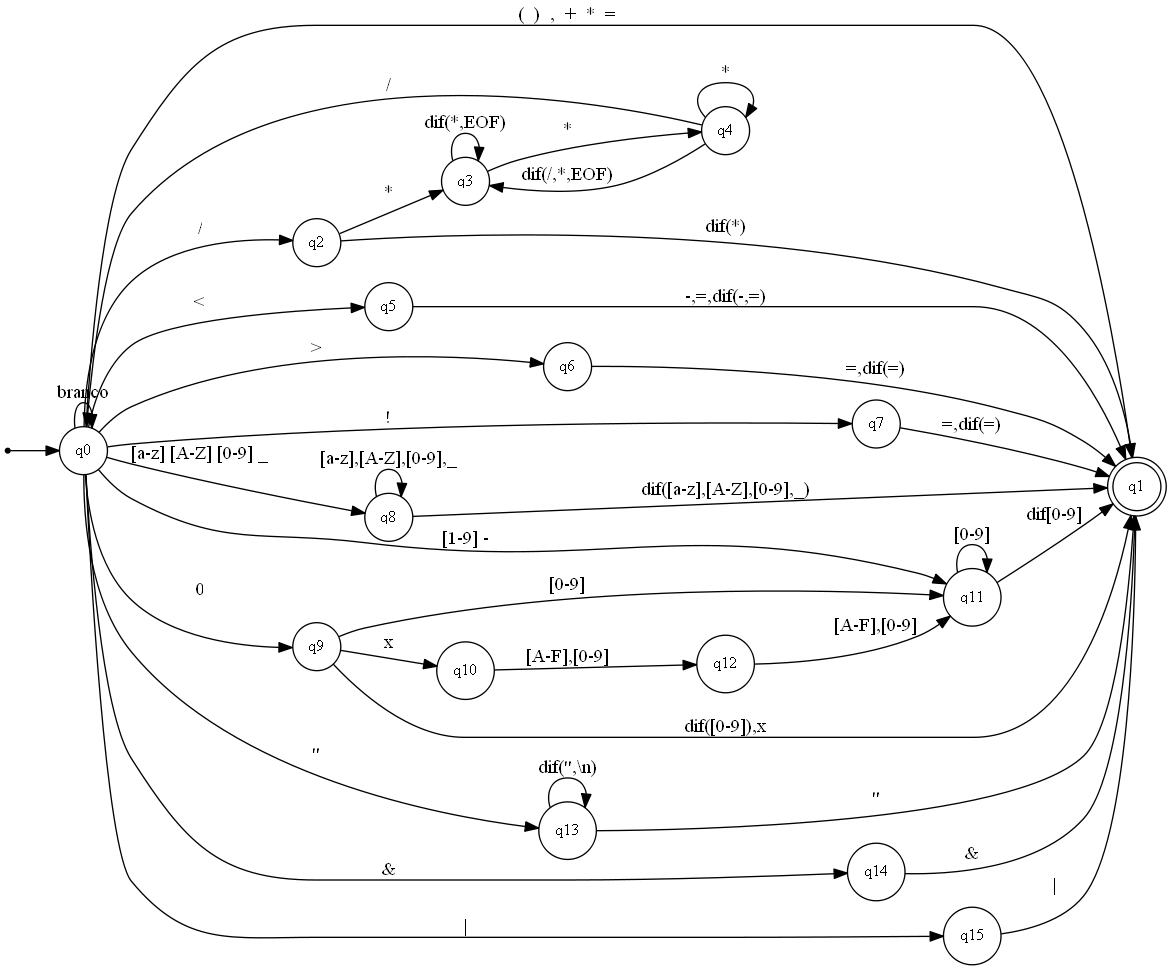
\includegraphics[width=0.9\textwidth]{figuras/automato.png}
	% Caption centralizada
	% Caption e fonte 
	 \vspace{0.2cm}
	\label{fig:figura1}
\end{figure}
\vspace{0.2cm}
\section{\esp Gramática com Expressões Regulares - GER}   
\begin{figure}[!ht]
	\vspace{0.2cm}
	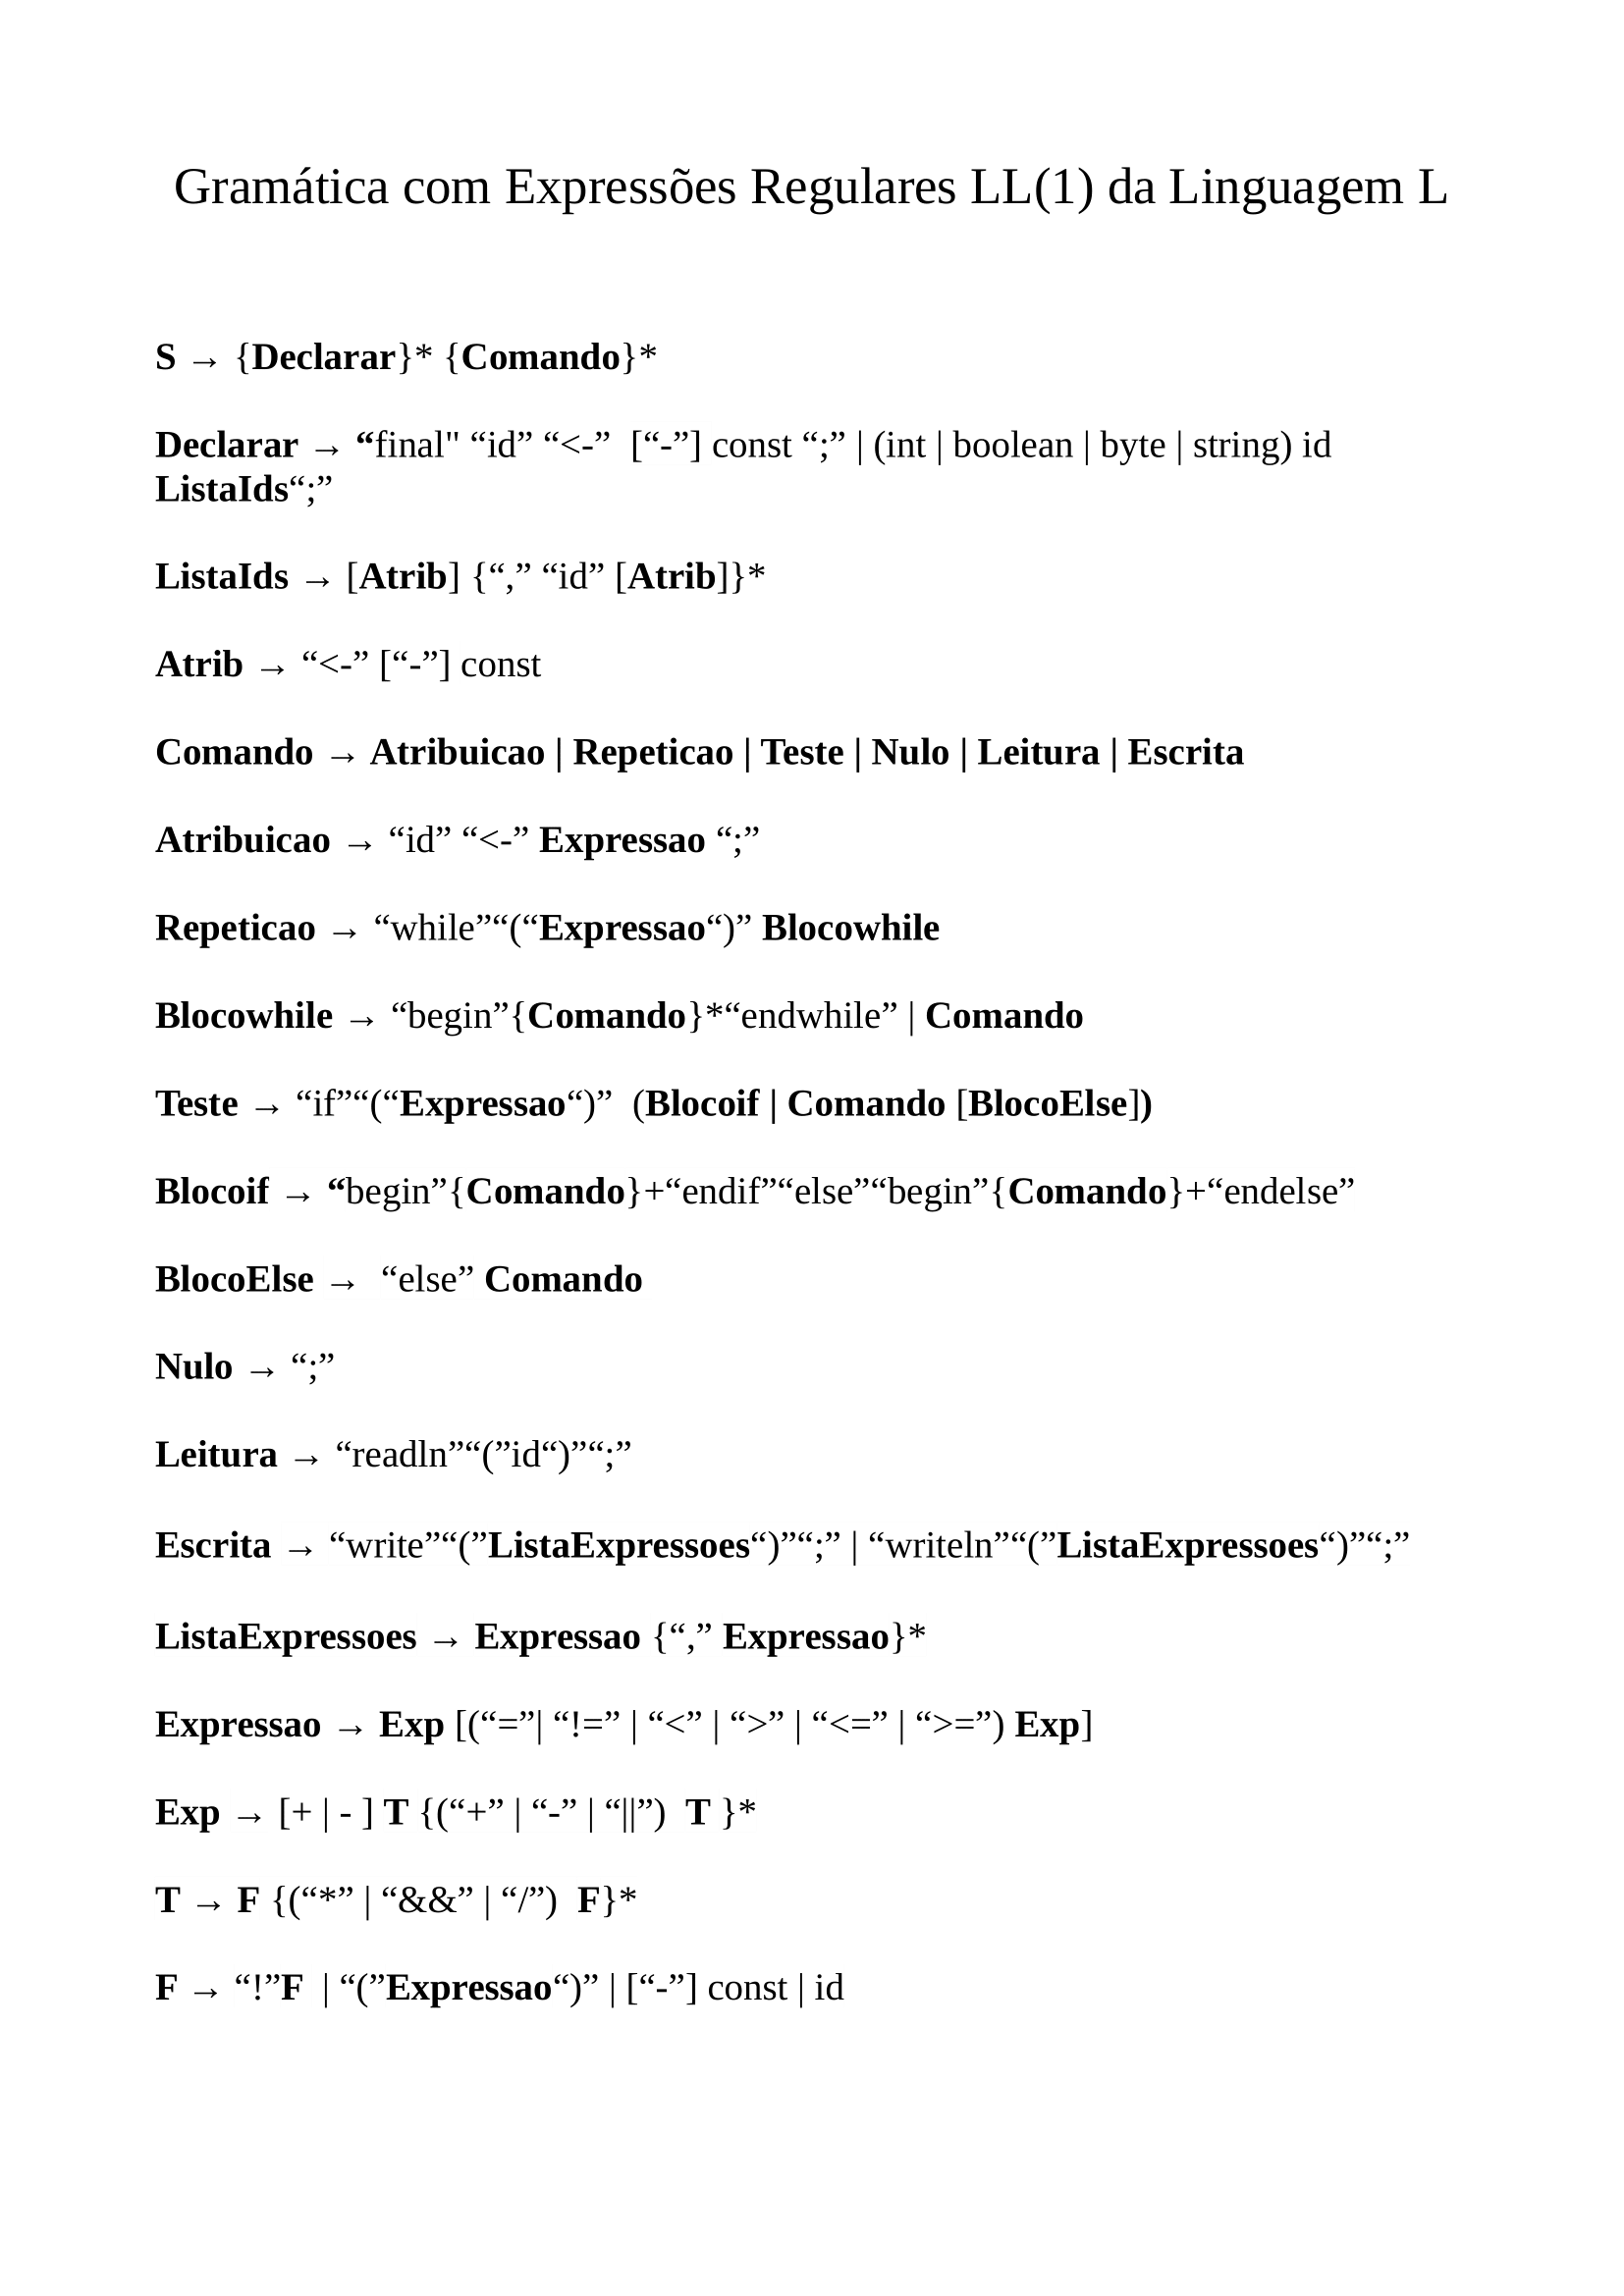
\includegraphics[width=0.9\textwidth]{figuras/GER_LL1-1.png}
	% Caption centralizada
	% Caption e fonte 
	 \vspace{0.2cm}
	\label{fig:figura1}
\end{figure}
\vspace{0.2cm}
\section{\esp Grámática Livre de Contexto - GLC}   
\begin{figure}[!ht]
	\vspace{0.2cm}
	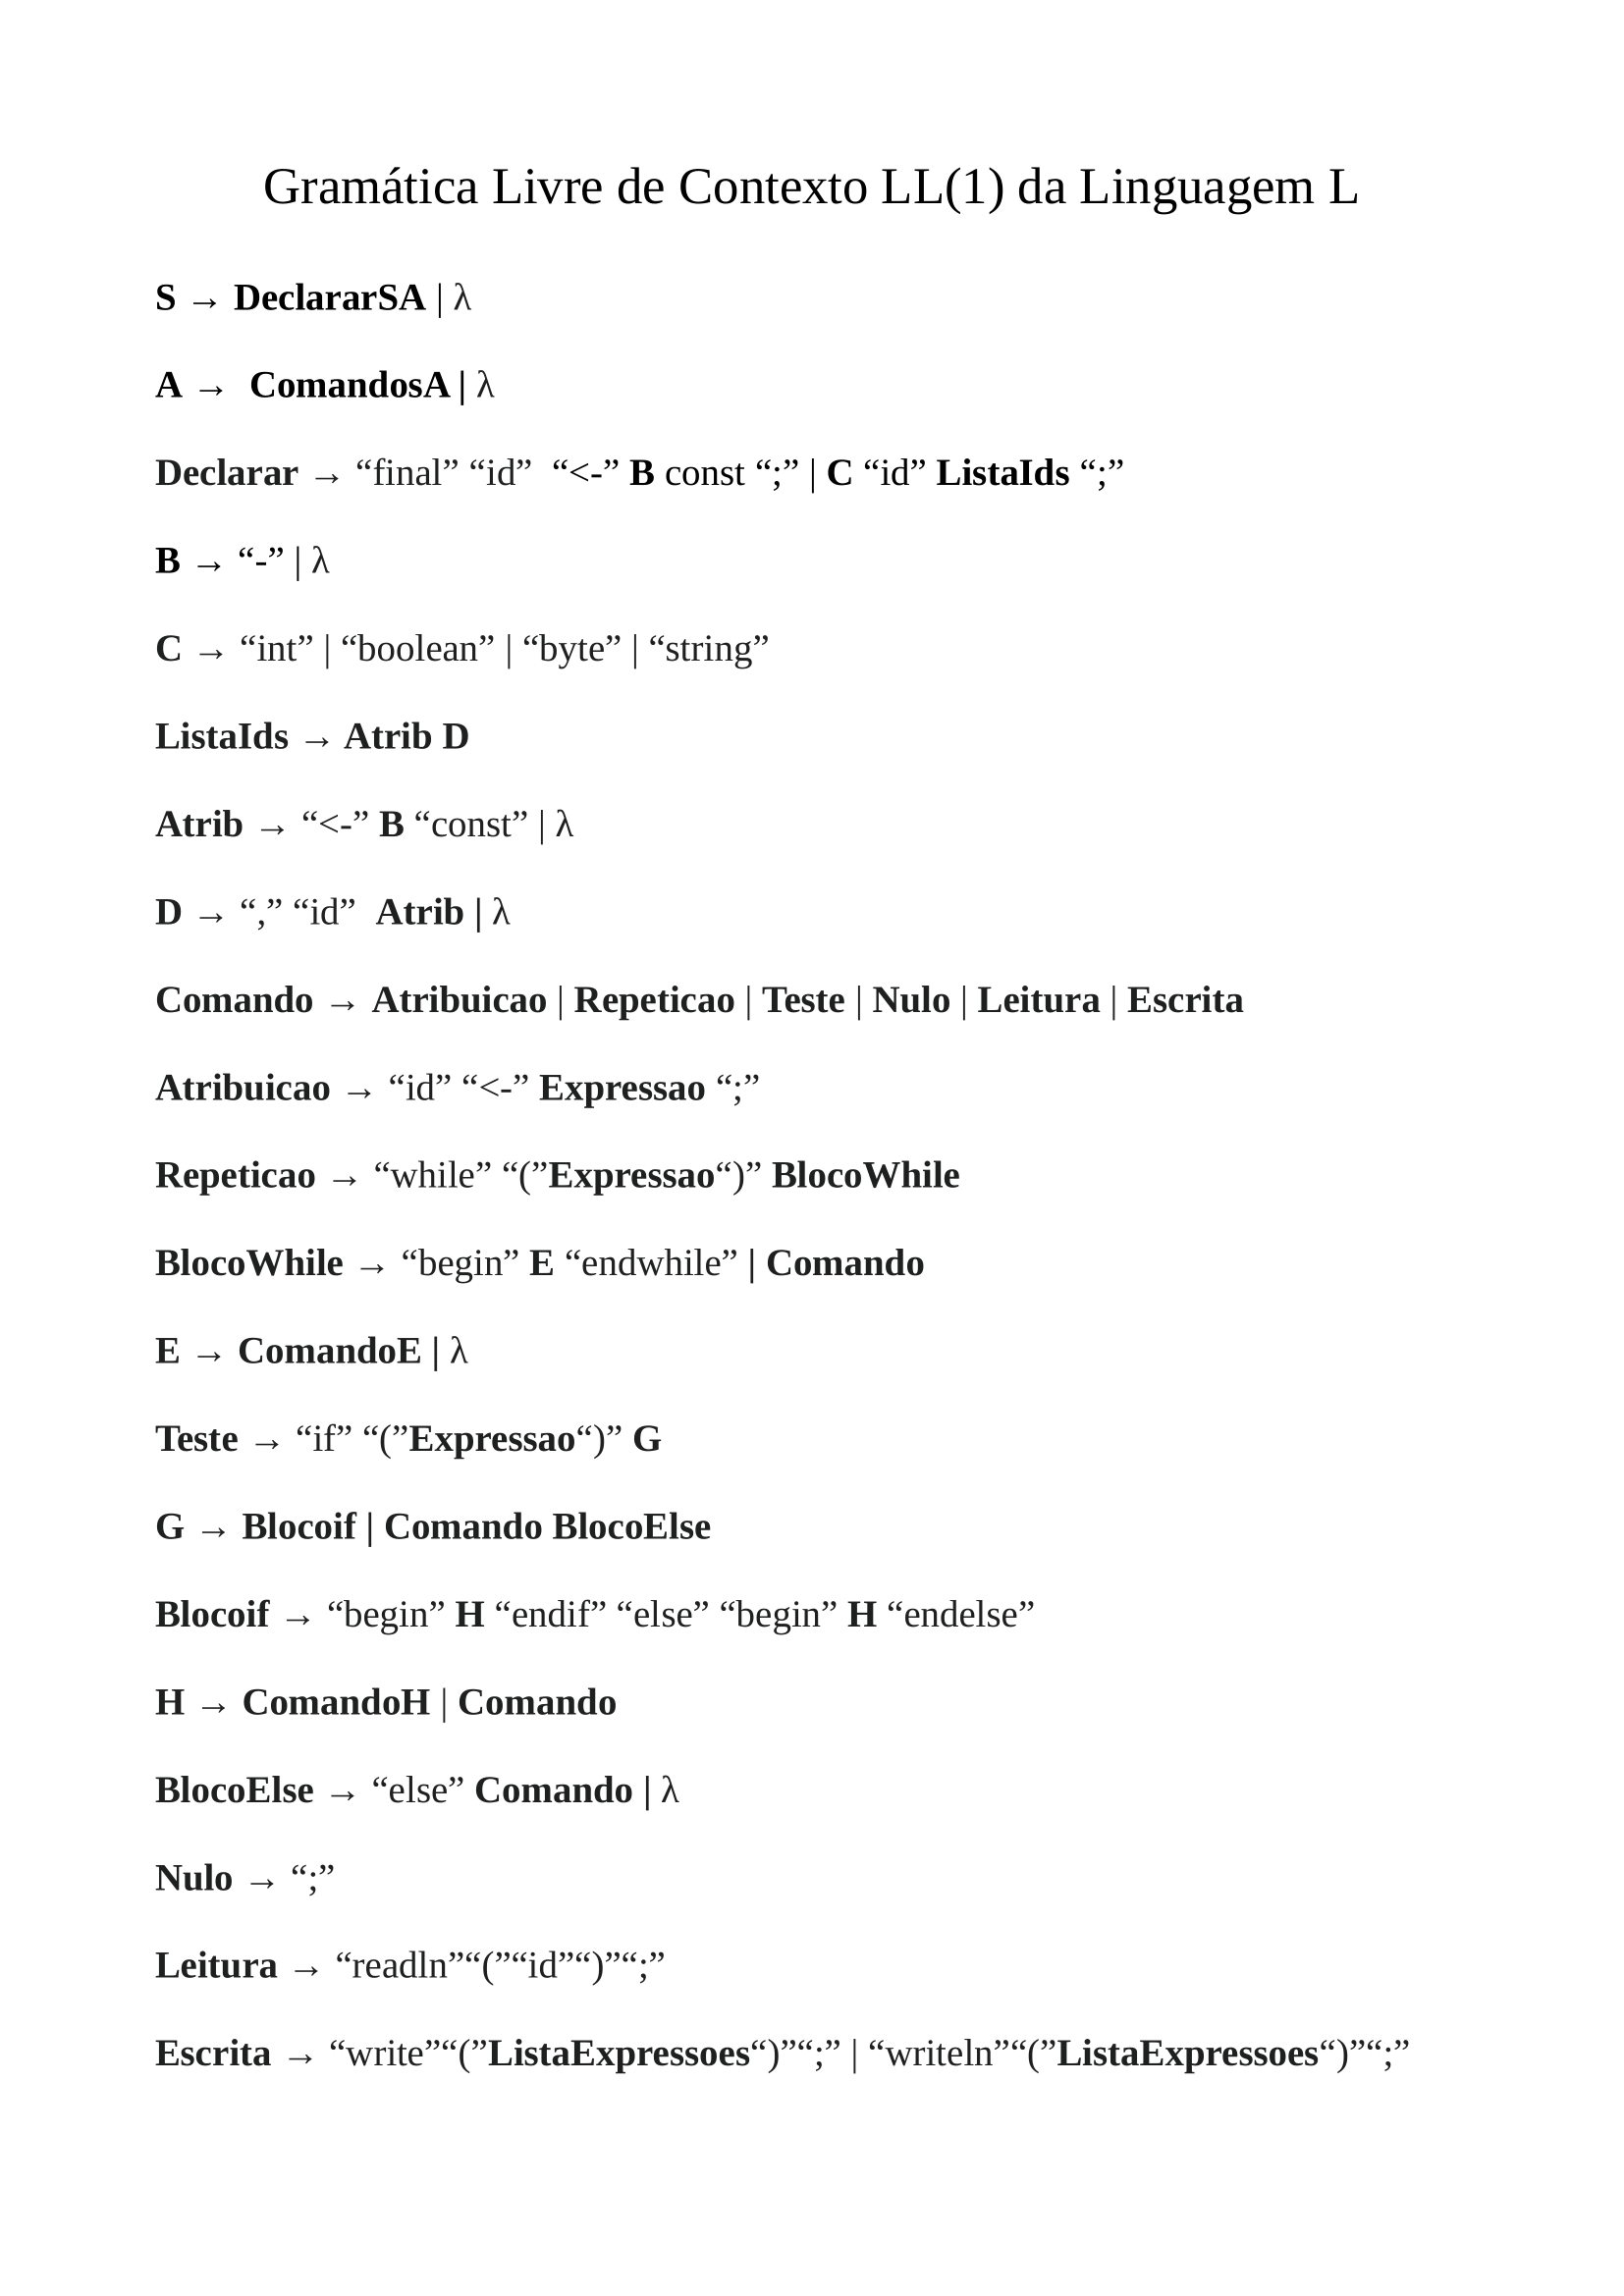
\includegraphics[width=0.9\textwidth]{figuras/GLC_LL1-1.png}
	% Caption centralizada
	% Caption e fonte 
	 \vspace{0.2cm}
	\label{fig:figura1}
\end{figure}

\begin{figure}[!ht]
	\vspace{0.2cm}
	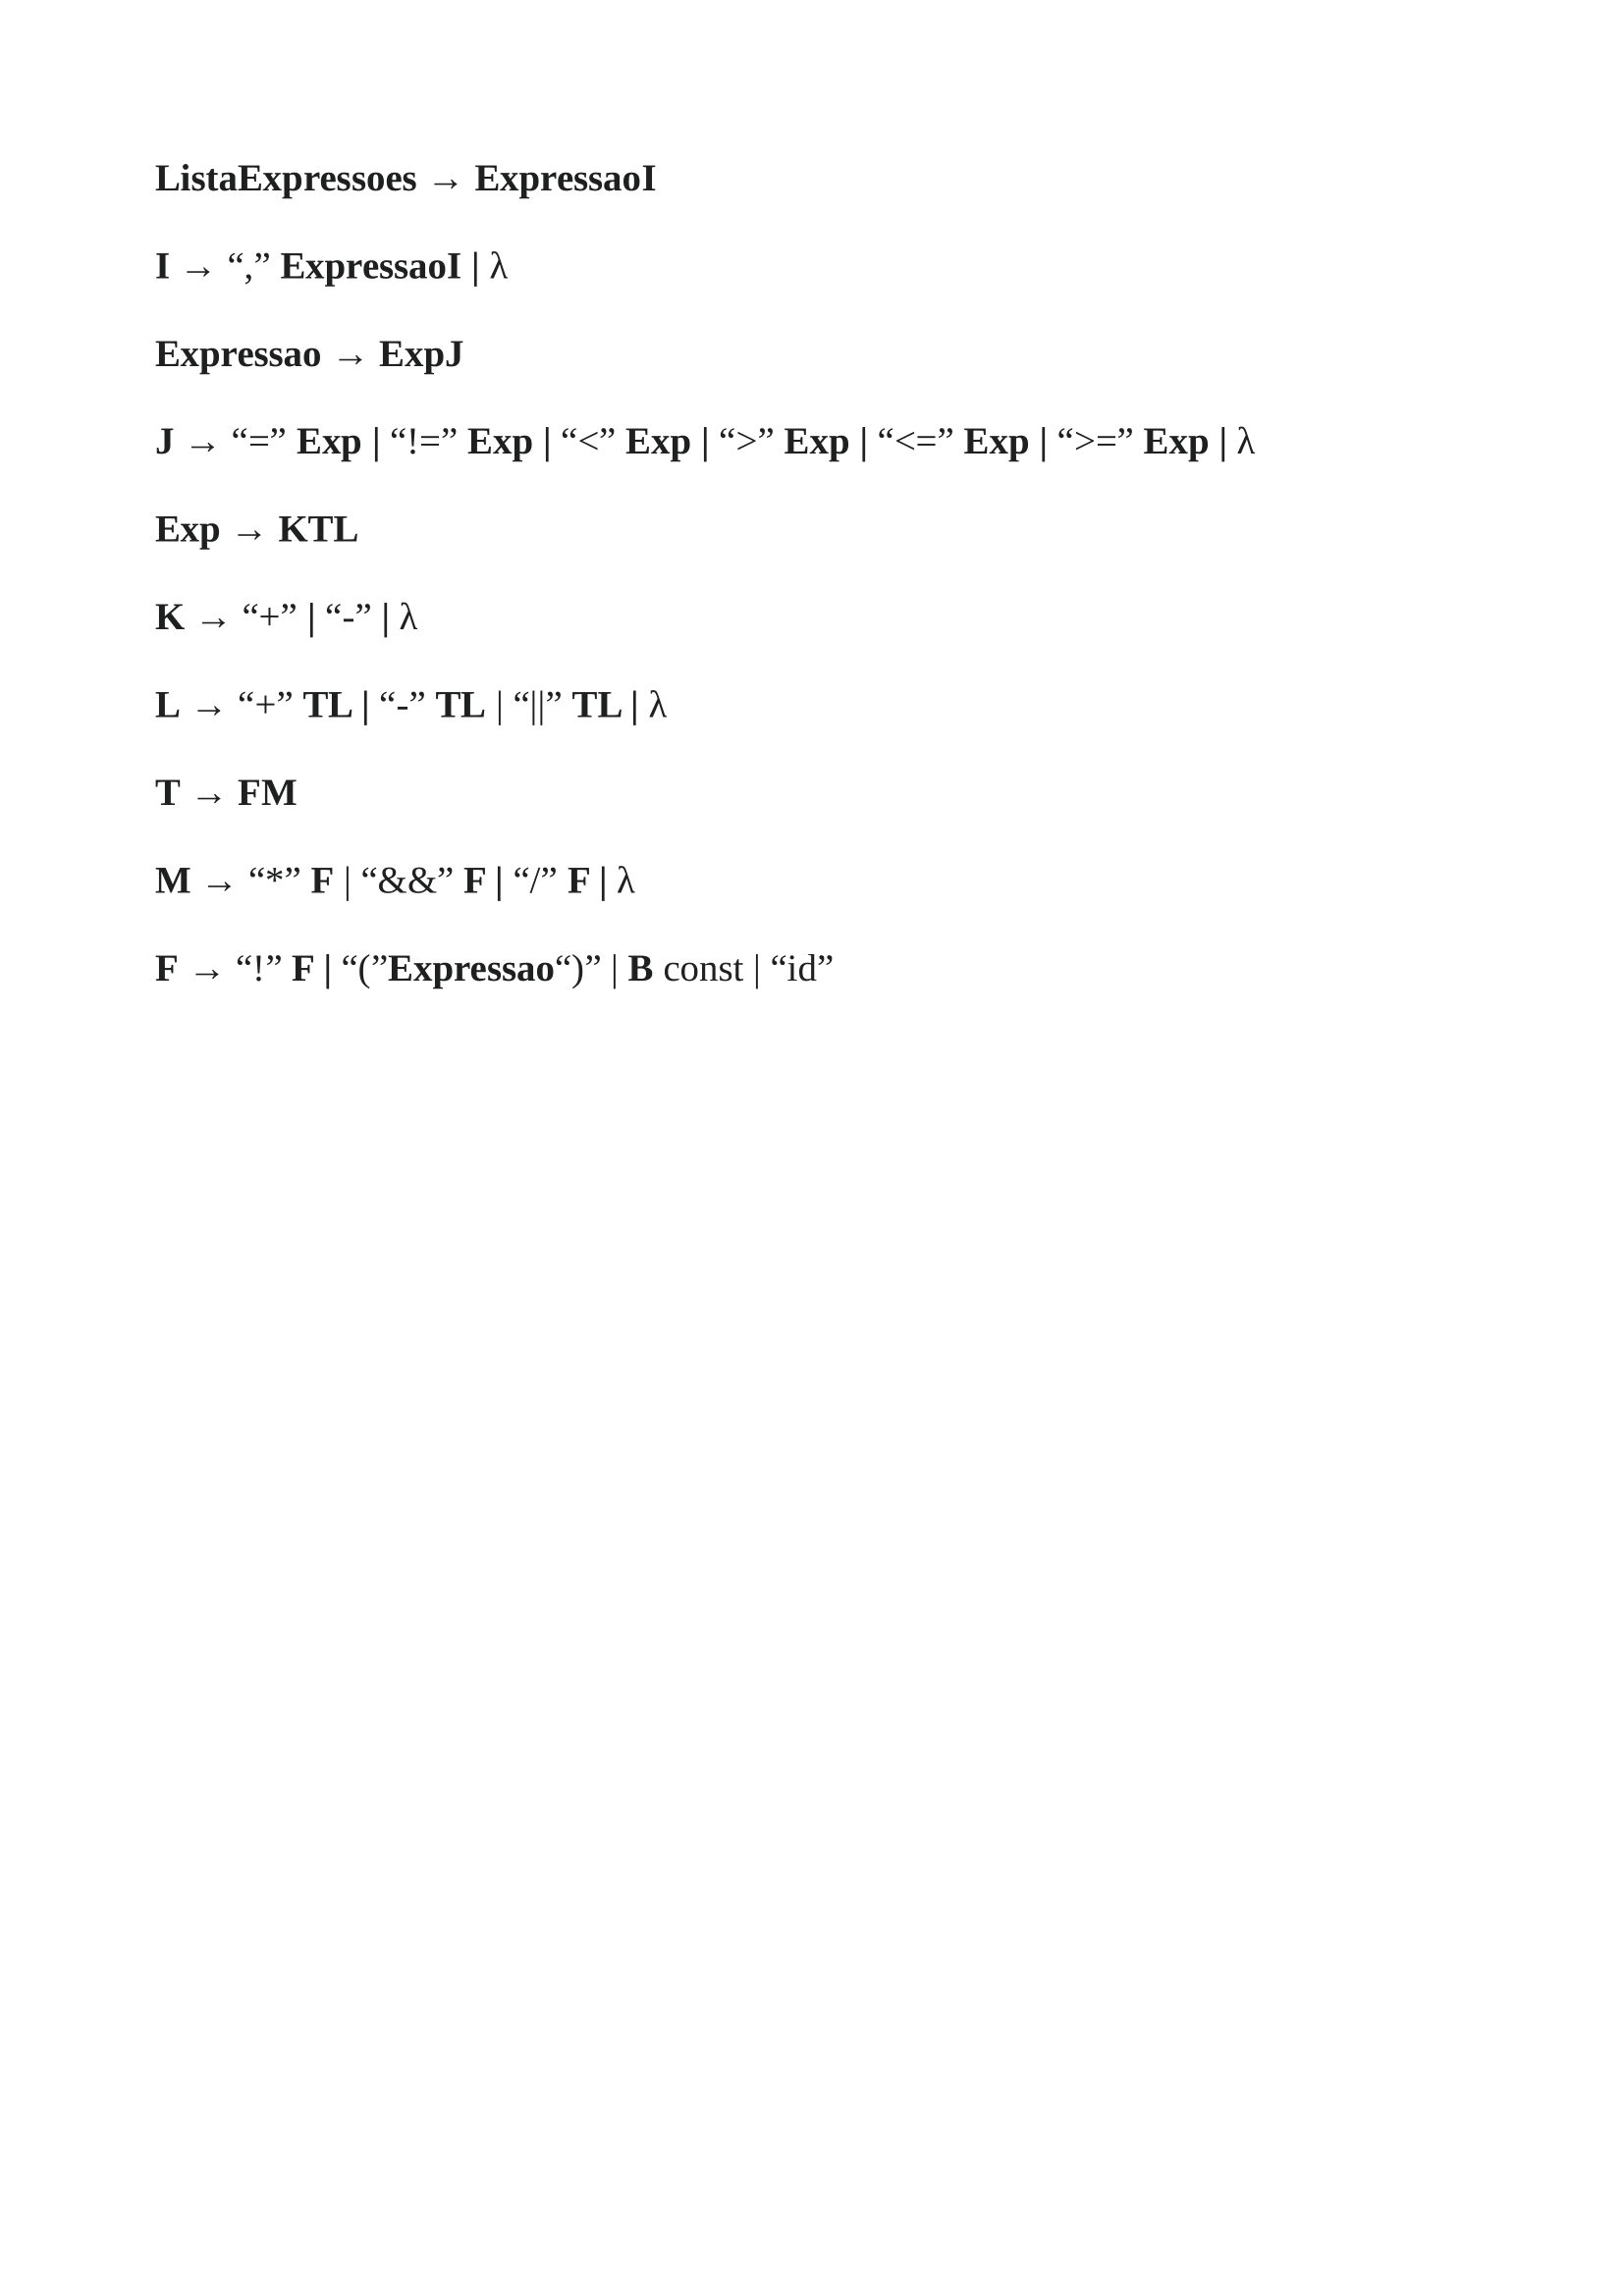
\includegraphics[width=0.9\textwidth]{figuras/GLC_LL1-2.png}
	% Caption centralizada
	% Caption e fonte 
	 \vspace{0.2cm}
	\label{fig:figura1}
\end{figure}
\vspace{0.2cm}


%%%%%%%%%%%%%%%%%%%%%%%%%%%%%%%%%%%
%% FIM DO TEXTO
%%%%%%%%%%%%%%%%%%%%%%%%%%%%%%%%%%%

% \selectlanguage{brazil}
%%%%%%%%%%%%%%%%%%%%%%%%%%%%%%%%%%%
%% Inicio bibliografia
%%%%%%%%%%%%%%%%%%%%%%%%%%%%%%%%%%%
\end{document}


